\documentclass[12pt, letterpaper, twoside]{article}\usepackage[]{graphicx}\usepackage[]{xcolor}
% maxwidth is the original width if it is less than linewidth
% otherwise use linewidth (to make sure the graphics do not exceed the margin)
\makeatletter
\def\maxwidth{ %
  \ifdim\Gin@nat@width>\linewidth
    \linewidth
  \else
    \Gin@nat@width
  \fi
}
\makeatother

\definecolor{fgcolor}{rgb}{0.345, 0.345, 0.345}
\newcommand{\hlnum}[1]{\textcolor[rgb]{0.686,0.059,0.569}{#1}}%
\newcommand{\hlstr}[1]{\textcolor[rgb]{0.192,0.494,0.8}{#1}}%
\newcommand{\hlcom}[1]{\textcolor[rgb]{0.678,0.584,0.686}{\textit{#1}}}%
\newcommand{\hlopt}[1]{\textcolor[rgb]{0,0,0}{#1}}%
\newcommand{\hlstd}[1]{\textcolor[rgb]{0.345,0.345,0.345}{#1}}%
\newcommand{\hlkwa}[1]{\textcolor[rgb]{0.161,0.373,0.58}{\textbf{#1}}}%
\newcommand{\hlkwb}[1]{\textcolor[rgb]{0.69,0.353,0.396}{#1}}%
\newcommand{\hlkwc}[1]{\textcolor[rgb]{0.333,0.667,0.333}{#1}}%
\newcommand{\hlkwd}[1]{\textcolor[rgb]{0.737,0.353,0.396}{\textbf{#1}}}%
\let\hlipl\hlkwb

\usepackage{framed}
\makeatletter
\newenvironment{kframe}{%
 \def\at@end@of@kframe{}%
 \ifinner\ifhmode%
  \def\at@end@of@kframe{\end{minipage}}%
  \begin{minipage}{\columnwidth}%
 \fi\fi%
 \def\FrameCommand##1{\hskip\@totalleftmargin \hskip-\fboxsep
 \colorbox{shadecolor}{##1}\hskip-\fboxsep
     % There is no \\@totalrightmargin, so:
     \hskip-\linewidth \hskip-\@totalleftmargin \hskip\columnwidth}%
 \MakeFramed {\advance\hsize-\width
   \@totalleftmargin\z@ \linewidth\hsize
   \@setminipage}}%
 {\par\unskip\endMakeFramed%
 \at@end@of@kframe}
\makeatother

\definecolor{shadecolor}{rgb}{.97, .97, .97}
\definecolor{messagecolor}{rgb}{0, 0, 0}
\definecolor{warningcolor}{rgb}{1, 0, 1}
\definecolor{errorcolor}{rgb}{1, 0, 0}
\newenvironment{knitrout}{}{} % an empty environment to be redefined in TeX

\usepackage{alltt}

\usepackage{amsmath}
\usepackage{booktabs}
\usepackage{amsthm}
\usepackage{graphicx}
\usepackage{lipsum}
\usepackage{listings}
\usepackage[margin=1.2in]{geometry}
\usepackage[colorlinks=true]{hyperref}
\hypersetup{colorlinks = true, linkcolor = blue, citecolor=blue, urlcolor = blue}
\usepackage{natbib}
\usepackage{enumitem}
\usepackage{setspace}
\graphicspath{ {/Users/patrickbrogan/Desktop/Manuscript/} }

\usepackage[pagewise]{lineno}
%\linenumbers*[1]
% %% patches to make lineno work better with amsmath
\newcommand*\patchAmsMathEnvironmentForLineno[1]{%
 \expandafter\let\csname old#1\expandafter\endcsname\csname #1\endcsname
 \expandafter\let\csname oldend#1\expandafter\endcsname\csname end#1\endcsname
 \renewenvironment{#1}%
 {\linenomath\csname old#1\endcsname}%
 {\csname oldend#1\endcsname\endlinenomath}}%
\newcommand*\patchBothAmsMathEnvironmentsForLineno[1]{%
 \patchAmsMathEnvironmentForLineno{#1}%
 \patchAmsMathEnvironmentForLineno{#1*}}%

 \AtBeginDocument{%
 \patchBothAmsMathEnvironmentsForLineno{equation}%
 \patchBothAmsMathEnvironmentsForLineno{align}%
 \patchBothAmsMathEnvironmentsForLineno{flalign}%
 \patchBothAmsMathEnvironmentsForLineno{alignat}%
 \patchBothAmsMathEnvironmentsForLineno{gather}%
 \patchBothAmsMathEnvironmentsForLineno{multline}%
}

\title{Country-Level Association Between Particulate Matter Air Pollution and Mortality}
\author{Patrick Brogan\\[1ex]
  Department of Statistics, University of Connecticut\\}
\IfFileExists{upquote.sty}{\usepackage{upquote}}{}
\begin{document}

\maketitle

\begin{abstract}
Air pollution has been consistently shown to be associated with mortality,
specifically respiratory morbidity. Identifying associations between specific
air pollutants and specific types of morbidity can inform future public health
practice and public environmental policy globally.The aim of this paper was to
build on this research with a contry-level analysis of the global effect of
PM2.5 pollution on three types of mortality: asthma, rheumatic heart disease,
and hypertensive heart disease. Using a linear mixed effects model to control
for covariates such as time, GDP per capita, and Sex, this paper found no
significant associations between average PM2.5 concentration and the age
standardized death rate from asthma, rheumatic heart disease or hypertensive
heart disease in each country.
\end{abstract}

\section*{Introduction}
\addcontentsline{toc}{section}{Introduction}
Air pollution is a serious public health and environmental issue, having been
linked to over 6.5 million global deaths each year \citep{fuller2022pollution}.
Previous research has demonstrated an association between air pollution and
mortality in specific localities or municipalities\citep{dockery1993association,
sunyer1996air, jerrett2005spatial, analitis2006short}. When talking specifically
about particulate matter, some studies have demonstrated an association between
particulate matter pollution and respiratory and cardiovascular deaths
\citep{analitis2006short}. However, other studies have found no significant
relationship between particulate matter pollution and the morbidity and
mortality rate \citep{khojasteh2021long}. The aim of this study is to analyze
the association between ambient PM2.5 air pollution in ppm and mortality from
asthma, rheumatic heart disease, and hypertensive heart disease at a country-wide
level rather than at the municipal level. Though previous literature analyzing
global air pollution and mortality has found significant associations between
the two, there has not yet been an analysis focusing specifically on ambient
PM2.5 air pollution and mortality from asthma, rheumatic heart disease, and
hypertensive heart disease globally. Using a linear mixed effects model to
account for the effects of sex, time, and GDP per capita, this study aims to
analyze the association between ambient PM2.5 concentration and mortality from
asthma, hypertensive heart disease, and rheumatic heart disease.

\section*{Data}
\addcontentsline{toc}{section}{Data}
The data for this analysis was compiled from the WHO's Ambient Air Quality
Database \citep{who2022airquality}, the WHO's Mortality Database
\citep{who2022all}, and the World Bank's data on GDP per capita, PPP
in constant 2017 international dollars \citep{worldbank2022}. The primary sources
for the air quality data were official reports of countries, official national
and subnational reports on measurements of PM10 or PM2.5 and ground measurements
compiled in the framework of the Global Burden of Disease project. Data reported
by Clean Air for Asia, the Air quality e-reporting database of the European
Environment Agency for Europe, the AirNow Programme from the United States
embassies and consulates, and values from peer-reviewed journals were also used.
The data on mortality comprise deaths registered in national vital registration
systems, with underlying cause of death as coded by the relevant national
authority. These data are official national statistics in the sense that they
have been transmitted to the World Health Organization by the competent
authorities of the countries concerned. The data on each country's GDP per
capita was compiled by the World Bank using each country's national accounts and
census data, using either the 1993 or 2008 System of National Accounts
Methodology. Since the data on ambient particulate matter pollution ranged from
2010 to 2016, this was the period that was analyzed for all datasets. The WHO
datasets on air quality and mortality help to answer for associations between
ambient PM2.5 air pollution and mortality from asthma, rheumatic heart disease,


\section*{Methods}
\addcontentsline{toc}{section}{Methods}
The three datasets were compiled into one dataframe in RStudio where all
statistical analyses were conducted. Since the air quality database only included
data from 2010 to 2016, only that time period was analyzed. The parameter estimated
is age standardized mortality rate in a given country from one of the three
specified mortalities and the explanatory variable is average country-wide
ambient PM2.5 concentration in ppm with the covariates being sex, time, and GDP
per capita. Instead of using a simple linear regression model, this study tests
for associations between nationwide PM2.5 air concentration and age standardized
mortality rates by using a linear mixed effects model which accounts for the
effects of sex, time, and GDP per capita such that:
\[
  MOR = \beta_{0} + \beta_{1}POL + \beta_{2}SEX + \beta_{3}TIME +\beta_{4}GDP
  + \beta_{5}(POL)(SEX) + \beta_{6}(POL)(TIME)
\]
\[
 + \beta_{7}(POL)(GDP) + E
\]
I did this using the lmer function in RStudio using the lme4 package in RStudio.
Running this model for the compiled dataframe yielded the point estimates for
the slopes and intercepts as well as the standard error for each. I was able to
find the p-values for each explanatory variable using the formula
\[
  p-value = 2(1 - \phi(|t-value|)
\]
where \begin{math}\phi(Z)\end{math} is the CDF of a standard normal random
variable.

\section*{Results}
\addcontentsline{toc}{section}{Results}
Using the linear mixed effect model with the given covariates, point estimates
for the slopes of each explanatory variable were obtained as well as the standard
error for each. Utilizing the given formula for the p-value, the significance of
each explanatory variable in predicting the response variable, age standardized
mortality rate per 100,000, was analyzed. After each of these processes were
conducted in order to control for covariates, no significant association was
found between a given country's average ambient PM2.5 air concentration and
the mortality rate from asthma, rheumatic heart disease, or hypertensive heart
disease. Although the regression for asthma was close to significance, a
p-value of 0.05655668, which is greater than the significance level of
\begin{math}\alpha = 0.05\end{math}. In that regression, GDP per capita and sex
were significant predictors of country-level death rate from asthma, as p-values
of \begin{math}6.591323\times10^{-3}\end{math} and
\begin{math}1.864832\times10^{-8}\end{math} were yielded respectively, though
time wasn't a significant predictor (p = 0.5332043). In the regression for
rheumatic heart disease, ambient PM2.5 air concentration and sex weren't
significant predictors of death rate with p-values of 0.5672925 and 0.1325090
respectively, but GDP per capita and time were, with p-values of
\begin{math}1.278235\times10^{-6}\end{math} and
0.2180579 respectively. In the regression for hypertensive heart disease,
ambient PM2.5 air concentration and time weren't significant predictors of death
rate with p-values of 0.3058979844 and 0.4970754156 respectively, but GDP per
capita and sex were, with p-values of 0.0005376261 and 0.0000000000 respectively.

\begin{figure}[t]
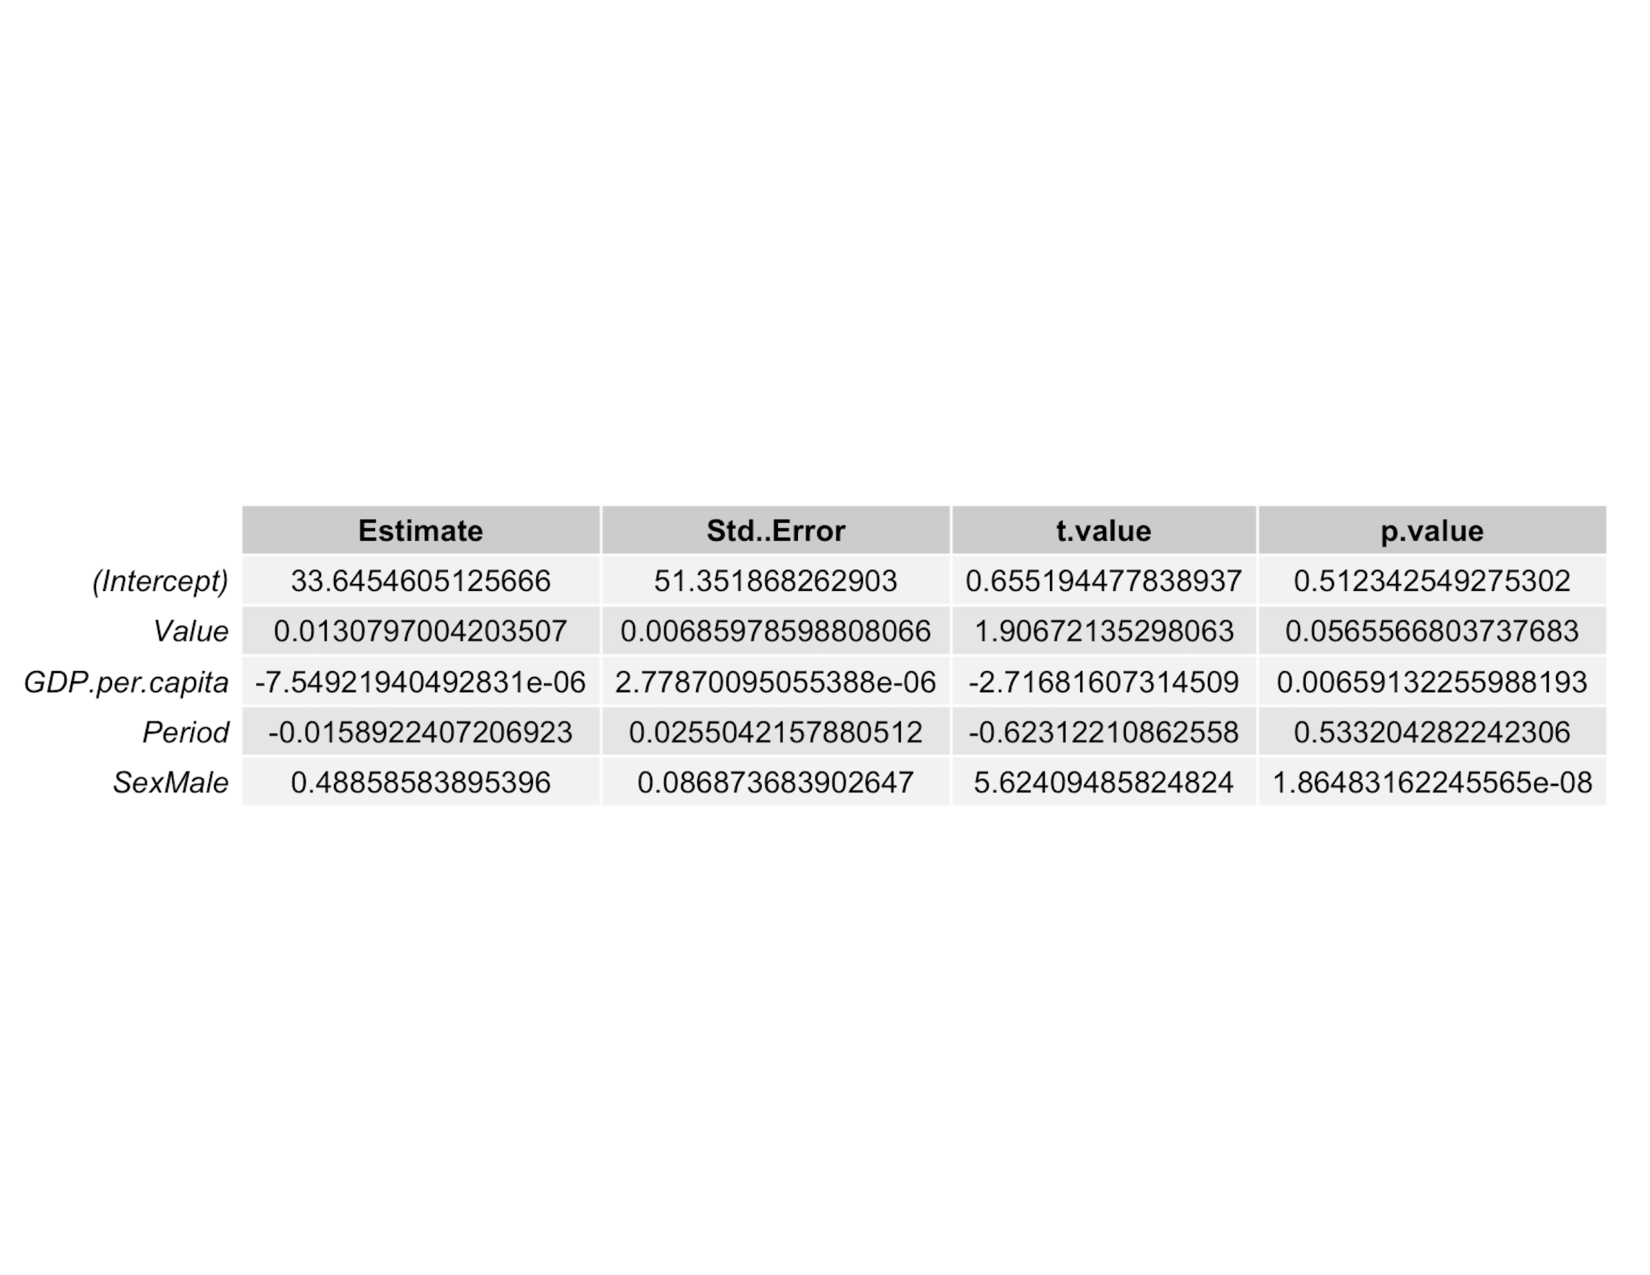
\includegraphics[scale=0.5]{asthma.chart.pdf}
  \centering
  \caption{Significance of explanatory variables on age standardized death rate
  from asthma in mixed effects model. PM2.5 pollution (Value) and Time (Period)
  aren't significant predictors but sex and GDP per capita are at the
  \begin{math}\alpha = 0.05\end{math} significance level.}
\end{figure}

\begin{figure}[t]
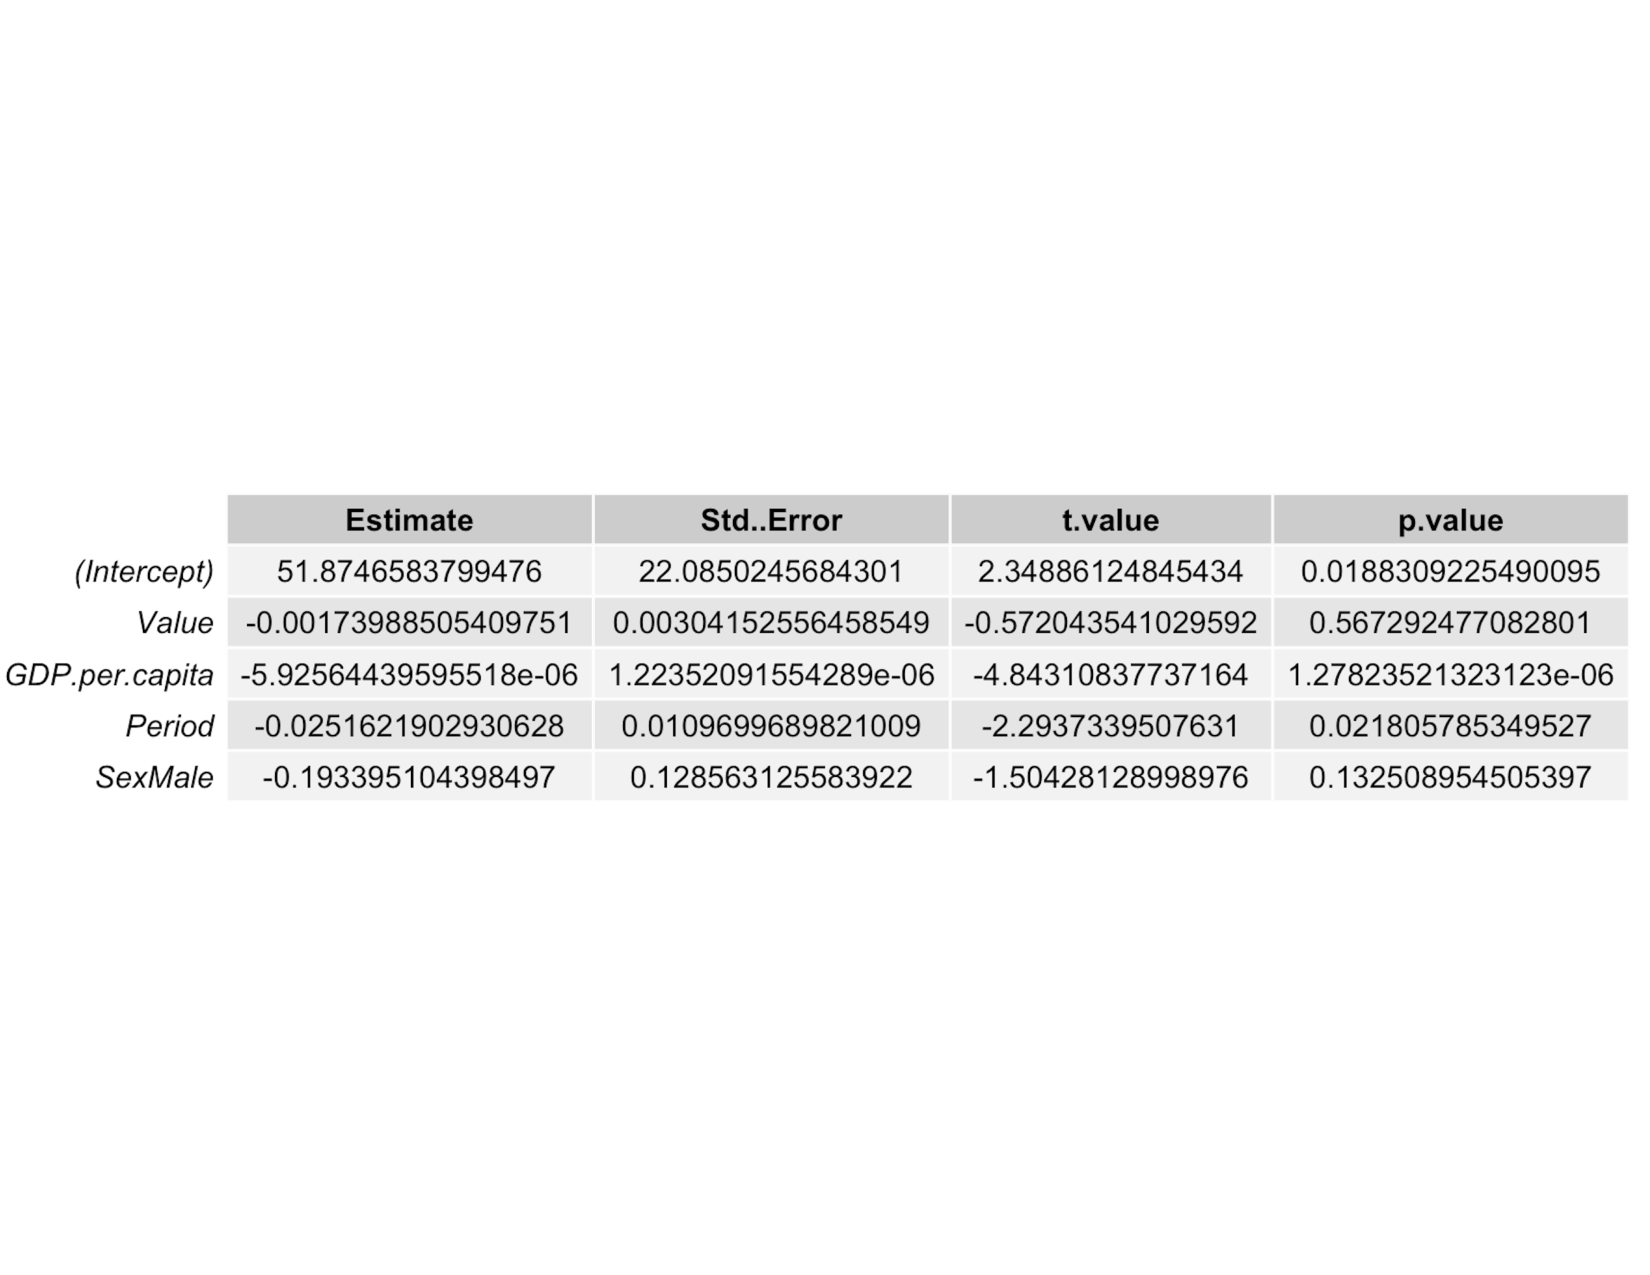
\includegraphics[scale=0.5]{rheum.chart.pdf}
  \centering
  \caption{Significance of explanatory variables on age standardized death rate
  from rheumatic heart disease in mixed effects model. PM2.5 pollution (Value)
  and Time (Period) aren't significant predictors but sex and GDP per capita are
  at the \begin{math}\alpha = 0.05\end{math} significance level.}
\end{figure}

\begin{figure}[t]
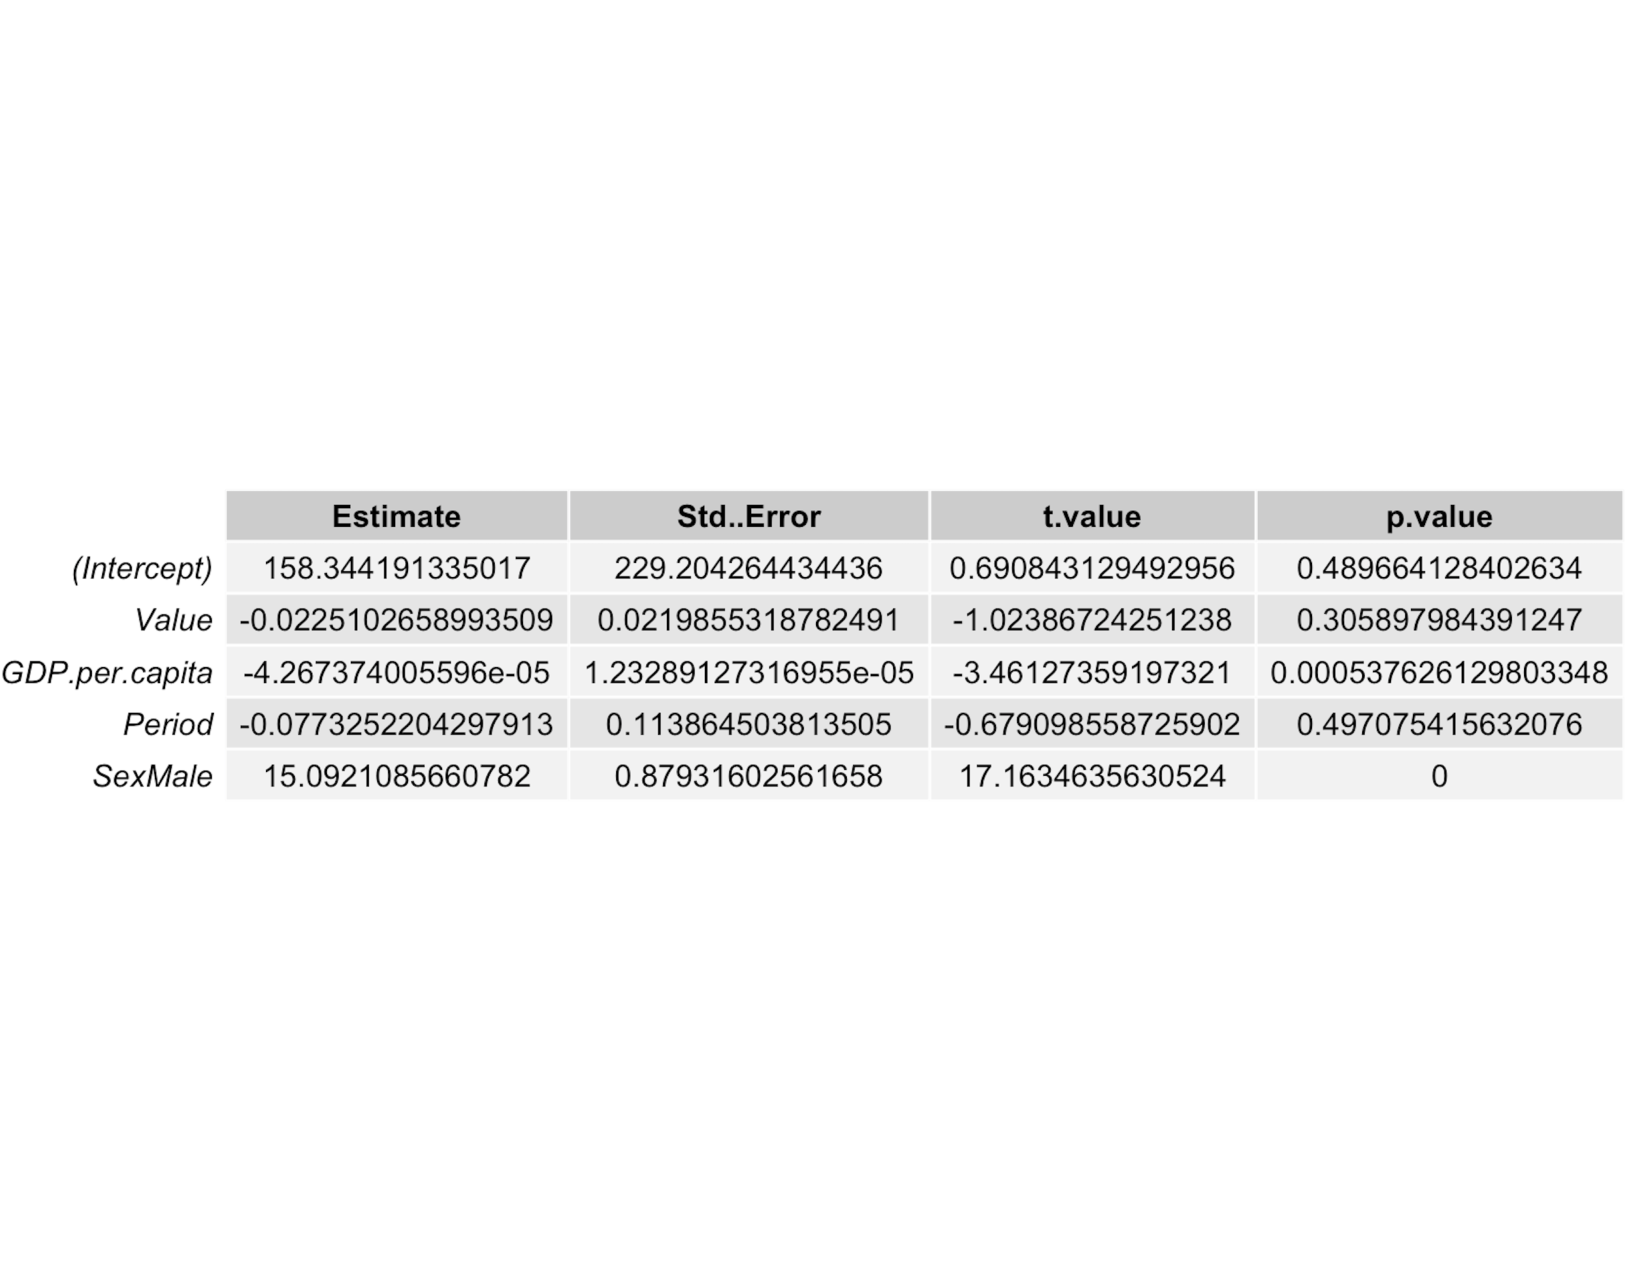
\includegraphics[scale=0.5]{hyper.chart.pdf}
  \centering
  \caption{Significance of explanatory variables on age standardized death rate
  from hypertensive heart disease in mixed effects model. PM2.5 pollution (Value)
  and sex aren't significant predictors but Time (Period) and GDP per capita are
  at the \begin{math}\alpha = 0.05\end{math} significance level.}
\end{figure}

\section*{Discussion}
The association between air pollution and mortality has been the topic of
scienticic inquiry for a long time, and many studies and analyses have been
conducted in order to elucidate the association between the two
\citep{dockery1993association, sunyer1996air, jerrett2005spatial, analitis2006short}.
The fact that air pollution contributes to over 6.5 million deaths every year
\citep{fuller2022pollution} makes this topic all the more consequential for
informing global public health and public policy practices. As mentioned before,
the research pertaining to ambient PM2.5 air pollution's association with
mortality has been equivocal, with some studies finding a significant association
\citep{analitis2006short} and others finding no such significant association
\citep{khojasteh2021long}. This study falls in the latter column, as no
significant association was demonstrated between a country's average ambient
PM2.5 air concentration and their age standardized death rate per 100,000 from
asthma, rheumatic heart disease, and hypertensive heart disease.
This study has several limitations. Firstly, data was only collected on the
average ambient PM2.5 concentration at the country level, and did not
differentiate between PM2.5 concentration levels in different regions or
localities. Similarly, the data collected on mortality rates in each country
only provided an average age standardized death rate for the entirety of each
country in the analysis. Due to the data having a much more broad and less
specific scope, the outcomes of the analyses may be affected. Secondly, the data
did not provide information about population density, so population density
was not accounted for in the analysis. Lastly, the data didn't include years
more recent than 2016, and this makes it so the results are not as relevant to
the current year, though the presence of COVID-19 may have skewed the mortality
rates from asthma, rheumatic heart disease or hypertensive heart disease. Despite
these limitations, this study adds to the plethora of literature that exists on
the subject of air pollution and mortality, helping to inform public health and
public policy in the future.

\bibliographystyle{STAT3494_refs}
\bibliographystyle{chicago}

\end{document}
